\PassOptionsToPackage{dvipdfmx}{graphicx}% NOTE: only for Japanese
\PassOptionsToPackage{dvipdfmx}{xcolor}% NOTE: only for Japanese
\documentclass[sip,biber]{now-journal}
\addbibresource{IEEEabrv.bib}
\addbibresource{ref.bib}

\usepackage[nolist,nohyperlinks]{acronym}
\usepackage{amsfonts}
\usepackage{bm}
\usepackage{mathtools}
\usepackage{interval}
\usepackage{siunitx}
\usepackage[skip=1pt]{subcaption}

% reload hyperref
\usepackage[colorlinks=true, allcolors=blue, plainpages=false, pdfpagelabels=true]{hyperref}
\usepackage{breakurl}

% cleveref setting
\usepackage[capitalise]{cleveref}
\crefformat{equation}{(#2#1#3)}
\Crefformat{equation}{#2Equation~(#1)#3}
\crefformat{section}{Section~#2#1{}#3}
\crefname{algorithm}{Algorithm}{Algorithms}
\crefname{equation}{}{}
\crefname{figure}{Figure}{Figures}
\crefname{section}{Section}{Sections}
\captionsetup[subfigure]{subrefformat=simple,labelformat=simple}
\renewcommand\thesubfigure{(\alph{subfigure})}
\def\crefrangeconjunction{--}

% psuedo codes
\usepackage{xcolor}
\usepackage[theorems,skins]{tcolorbox}
\usepackage{tabularx}
\usepackage{pseudo}
\newtcbtheorem[crefname = {Algorithm}{algorithms}]{algorithm}{Algorithm}{pseudo/booktabs, float=t, theorem hanging indent=0pt}{alg}
\pseudodefinestyle{fullwidth}{
    begin-tabular=
    \tabularx{\textwidth}[t]{@{}
        r                                          % Labels
        >{\leavevmode\pseudosetup}                 % Indent, font, ...
        X                                          % Code (flexible)
        >{\leavevmode} % Comment styling
        p{0.20\textwidth}                           % Comments (fixed)
        @{}},
    end-tabular=\endtabularx,
}
\pseudoset{%
   fullwidth,
   kwfont=\sffamily\bfseries,
   font=\kwfont,
   prfont=\textsf,
   hsep=0em,
   indent-mark,
   indent-mark-color=gray,
   indent-mark-shift=.5em,
   indent-length=2.0em,
   line-height=1.4,
   ct-left=\hfill\texttt{//}~,
   ct-right=,
   % label=\textcircled{\ttfamily\scriptsize\arabic*},
   label=,
   % ref,
}

% Align euqality or replacement in pseudo codes
% ref: https://latex.org/forum/viewtopic.php?t=26363
\usepackage{xparse}
\DeclareDocumentCommand{\psm}{m O{$\gets$}}{% pseudocode-math
  {\hphantom{$W_{k,f,t - 1}$}\llap{#1}~#2}%
  % {\rlap{#1}\hphantom{$W_{k,f,t}$}#2}%
}

% Original style files
\usepackage{bsssym}
\newcommand{\todo}[1]{\textcolor{red}{#1}}

% Document information
\title{Self-Rotation-Robust Online Independent Vector Analysis with\\Sound Field Interpolation on Circular Microphone Array}
\fancyhead[LO]{\footnotesize\textit{Self-rotation-robust online independent vector analysis with sound field interpolation on circular microphone array}}
\author{Nakashima, Taishi}
\affil{Tokyo Metropolitan University, Tokyo, Japan}
\author{Wakabayashi, Yukoh}
\affil{Toyohashi University of Technology, Aichi, Japan}
\author[1]{Ono, Nobutaka}
\creditline{%
  Corresponding author: Taishi Nakashima, \href{mailto:taishi@ieee.org}{taishi@ieee.org}.
  This work was supported by JSPS KAKENHI Grant Number 21J22039 and JST CREST Grant Number JPMJCR19A3.
}

\articledatabox{
  Received XX June 2023; Revised YY Sep 2023
  ISSN XXXX-YYYY; DOI xx.yyyy/zzz.wwwwwwww\\
  \copyright 2023 T. Nakashima, Y. Wakabayashi, and N. Ono
}

\keywords{
  Blind source separation,
  online independent vector analysis,
  circular microphone array,
  sound field interpolation
}

\begin{document}

\begin{abstract}
  % 本論文では,マイクロホンアレイの回転に頑健なオンラインブラインド音源分離手法を提案する.
  % Online auxiliary-function-based independent vector analysis (OIVA)はリアルタイムBSSを実現するための有望な手法のひとつである.
  % リアルタイムBSSを実用化するためには,音源やマイクの移動といった環境の変化に対する頑健性が重要な課題である.
  % 一般的にリアルタイム処理の最中に環境の変化が起こった場合はパラメータの再推定が必要である.
  % OIVAでは音源のなめらかな移動に対して頑健かつ高い分離性能を獲得できることが示されていた.
  % しかし,OIVAはマイクの突発的な移動に対しては十分な性能が得られない.
  % そこで本論文では,円状等間隔マイクロホンアレイ(CMA)のための音場補間処理を利用したOIVAを提案する.
  % 音場補間はCMAの回転を打ち消し,パラメータの再推定を必要とせずにBSSを可能にする.
  % 我々は,SFIを前処理として組み合わせた単純な手法と,適切なパラメータ変換を用いたより実応用な手法の2つを提案する.
  % シミュレーション実験の結果は音場補間によりマイクが回転する状況における音源分離の頑健性が向上したことを確認した.
  In this paper, we propose an online blind source separation (BSS) method robust against the self-rotation of microphone arrays.
  Online auxiliary-function-based independent vector analysis (OIVA) is one of the promising methods for real-time BSS.
  One major issue for real-time BSS is robustness against the movement of the source or microphone.
  Parameter re-estimation is necessary if such changes occur during processing.
  OIVA is robust against smooth movement of sources and achieves high separation performance.
  However, OIVA could perform better against rapid movements of microphones.
  This paper exploits sound field interpolation (SFI) for circular microphone arrays (CMAs) with OIVA.
  SFI cancels out the rotation of the CMA, enabling us to apply BSS without parameter re-estimation.
  We propose two methods; a combination of SFI and OIVA as a pre-processing and a method using parameter transformations for practical applications.
  Simulation experiments confirmed that SFI improves the robustness of the OIVA in situations where the microphone is rotating.
\end{abstract}

\section{Introduction}\label{sec:intro}
% ブラインド音源分離は混合信号から目的の信号を分離する技術である.
% BSSの手法はIVAやその拡張などが有名である.
% これらの手法はすべて時不変な系を仮定している.
% それに対して,実応用のためにはマイクロホンや音源の移動など系の時間変化を考慮する必要がある.
% 系の時間変化を考慮するためには,信号を短いブロックに分割し,各ブロックに対してIVAを適用するやり方が考えられる.
Blind source separation (BSS) \cite{Makino:2018:ASS} is a technique to extract the source signals from their observed mixture.
Popular approaches for BSS include independent vector analysis (IVA) \cite{Kim:2006:ASLP,Hiroe:2006:ICA}, auxiliary-function-based IVA (AuxIVA) \cite{Ono:2011:WASPAA}, and its extensions \cite{Kitamura:2016:ASLP,Nugraha:2020:SPL,Brendel:2020:SP}.
These methods assume a time-invariant acoustic transfer system (ATS).
However, in practical applications, considering time variations of the ATS, such as microphone movements, is necessary.

% 近年,動的な環境を考慮したマルチチャネル音響信号処理が注目されている.
% これまでに,recursiveなパラメータ更新を用いた beamforming, doa estimation, speaker tracking などが提案されてきた.
% さらに,動的な環境下における音声処理を題材としたコンペティションも開催され,データセットの整備も進められている.
% Clarity Challengeは補聴器の音声明瞭度向上のためのチャレンジであり,聴取者の頭の動きのデータも含まれている.
% SPEAR challengeでは,頭部装着型のヒアラブルデバイスのための音声強調チャレンジであり,話者や頭の動きのデータを含んだ広範なデータセットが配布されている.
Multi-channel acoustic signal processing techniques considering the dynamic environment have attracted much attention recently.
Several methods using recursive parameter updates have been proposed, such as beamforming \cite{Higuchi:2017:ASLP}, DOA tracking \cite{Weisberg:2019:ICASSP}, and speaker tracking \cite{Schwartz:2021:ASMP}.
Furthermore, competitions have been organized, and datasets developed on speech processing in dynamic scenarios.
Clarity Challenge \cite{Akeroyd:2023:ICASSP} aims to improve speech intelligibility in hearing aids and includes data on the listeners' head movements.
SPEAR Challenge \cite{Guiraud:2022:IWAENC} is a speech enhancement challenge for head-worn hearable devices, and extensive datasets called EasyCom \cite{Donley:2021:arxiv} have been distributed that include a speaker and head movement data.

% ブロックバッチの手法やオンラインの手法が考えられる.
% 特に,オンライン独立ベクトル分析は実時間で動作し,高い性能を示した.
% オンラインAuxIVA は補聴器への応用,残響除去との組み合わせ,高速なステアリングベクトル更新など最近活発に研究されている.
% オンラインAuxIVA ではフレームごとに分離行列を推定し,音響伝達系のゆるやかな時間変化に対応できる.
% しかし,新たな音源の出現やマイクの移動など,音響伝達系の突発的な変化が起こった場合には推定が難しくなり性能が著しく低下する.
In the context of BSS, many methods have been proposed based on block batch \cite{Koldovsky:2019:ICASSP,Koldovsky:2021:SP,Jansky:2022:ASMP} or online processing \cite{Kim:2010:CASI,Taniguchi:2014:HSCMA} to account for environmental changes.
In particular, online AuxIVA (OIVA) shows high separation performance in real-time scenarios \cite{Taniguchi:2014:HSCMA}.
It also has been actively researched recently for applications in hearing aids \cite{Sunohara:2017:ICASSP}, joint optimization with dereverberation \cite{Ueda:2021:ICASSP}, and computationally efficient optimization \cite{Nakashima:2023:ICASSP}.
OIVA estimates demixing matrices frame-by-frame manner and can track smooth environmental changes in ATS, such as slow movements of sources.
However, rapid changes in ATS, such as the emergence of new sources or microphone movement, make online BSS difficult and thus degrade separation performance.

% 音響伝達系の突発的な変化に対応するための音響信号処理手法がいくつか提案されている.
% 円状等間隔マイクロホンアレイ(circular microphone array; CMA)の回転を考え,音場の補間により対応する手法が提案されている.
% この手法はCMAの対称性を利用することで,CMAが回転する前の音場を簡単な線形演算により推定する.
% また,ビームフォーミング \cite{Wakabayashi:2021:ICASSP} やステアリングベクトル推定 \cite{Wakabayashi:2021:ASJ:A} への応用や,
% CMAの回転角度を自己推定する手法 \cite{Lian:2021:APSIPA} も提案されている.
% オンラインBSSとSFIを組み合わせれば,マイクの回転に対する頑健性を向上させられると期待できる.
Several methods have been proposed to cope with such rapid changes.
Sound field interpolation (SFI) for circular microphone array (CMA) has been proposed to address the rotation of a CMA \cite{Wakabayashi:2023:ASLP}.
This method exploits the symmetry of the CMA to estimate the sound field before the rotation of the CMA by a simple linear operation.
Applications to beamforming \cite{Wakabayashi:2021:ICASSP} and steering vector estimation \cite{Wakabayashi:2021:ASJ:A} have also been proposed,
as well as a method for self-estimating the rotation angle of a CMA \cite{Lian:2021:APSIPA}.
We expect the combination of OIVA and SFI to improve the robustness against the rotation.

In this paper, we address BSS in situations where a CMA rotates.
SFI cancels out the effect of the rotation, and BSS is applied in the latter stage.
As described in \cref{sec:proposed}, a naive combination of SFI and OIVA has a problem for practical applications.
In contrast, this study introduces a more straightforward method than that and demonstrates its effectiveness through experiments.
Experiments show that our proposed scheme is significantly better than the conventional OIVA.

The rest of this paper is organized as follows.
We formulate our motivation in \cref{sec:problem}.
\Cref{sec:conventional} describes online BSS, SFI, and how to combine them.
In \cref{sec:proposed}, we propose a new online BSS that utilizes the information before and after the rotation of CMA.
We conduct some experiments to show the efficacy of the SFI for online BSS in \cref{sec:experiment}.
\Cref{sec:conclusion} concludes this paper.

\section{Problem Formulation}\label{sec:problem}
\begin{figure}[t]
  \centering
  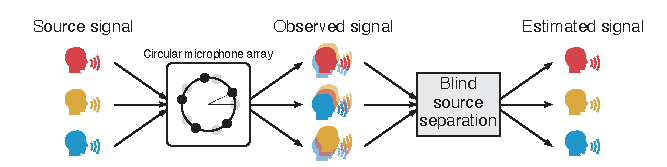
\includegraphics{figures/diagrams/bss.pdf}%
  \caption{Overview of blind source separation problem with a circular microphone array.}%
  \label{fig:bss}
\end{figure}
Let us consider the BSS problem with a CMA that can be horizontally rotated as shown in \cref{fig:bss}.
Let $\Src$ and $\Mic$ be the number of sources and microphones, respectively.
We assume that the observed signal $\Obs _{\ft}$ is in the short-time Fourier transform (STFT) domain modeled as
\begin{equation}
  \Obs _{\ft} = \steer _{1,\ft} \sig _{1,\ft} + \dots + \steer _{\Src,\ft} \sig _{\Src,\ft} = \sum _{\src=1} ^{\Src} \steer _{\src,\ft} \sig _{\src,\ft},\label{eq:mix}
\end{equation}
where $\freq = 1, \dots, \Freq$ denotes the frequency bin index,
$\tframe = 1, \dots, \Tframe$ denotes the time frame index,
$\sig _{\src,\ft} \in \C\; (\src = 1, \dots, \Src)$ denotes the $\src$th source signal,
and $\steer _{\src,\ft} \in \C ^{\Mic}$ denotes the steering vector of the $\src$th source signal to each microphone.
Also, we here set the \emph{reference microphone} $\refmic = 1$ without loss of generality.
In this case, each steering vector can be denoted as
\begin{equation}
  \steer _{\src,\ft} \coloneqq \begin{bmatrix} 1 & \str _{2,\src,\ft} & \dots & \str _{\Mic,\src,\ft} \end{bmatrix} ^{\top}\; (\src = 1, \dots, \Src).
\end{equation}
Under this definition, $\str _{\mic,\src,\ft} \; (\mic = 2, \dots, \Mic,\; \forall \src = 1, \dots, \Src)$ corresponds to the relative transfer function from the $\src$th source to the $\mic$th microphone, and thus each source signal $\sig _{1,\ft},\, \dots,\, \sig _{\Src,\ft}$ can be regarded as the \emph{source image} at the reference microphone.
Note that many BSS methods require a time-invariant mixing system $\steer _{\src,\freq}\; (\forall \src)$,
whereas, in this paper, steering vectors are time-variant $\steer _{\src,\ft}\; (\forall \src)$ to account for CMA rotations.
We aim to estimate source images at the reference microphone even if the CMA is rotated.
In the following, we assume that the rotation angle $\theta_t$ at each frame is available by another sensor.

Next, we consider an online BSS problem with the model defined above.
We henceforth assume that the number of microphones of CMA is equal to that of sources; $\Mic = \Src$.
\renewcommand{\Mic}{\Src}%
We aim to estimate demixing matrices and estimated signals using only the current and past observed signals $\Obs _{\freq,1},\, \dots,\, \Obs _{\freq,\tframe}$:
\begin{align}
  \Demix _{\ft} &= \begin{bmatrix} \demix _{1,\ft} & \dots & \demix _{\Src,\ft} \end{bmatrix} ^{\hermite} \in \C ^{\Src \times \Mic}, \\
  \Est _{\ft} &= \Demix _{\ft} \Obs _{\ft} \in \C ^{\Src},\label{eq:bss:sep}
\end{align}
where $\Demix _{\ft}$ is the demixing matrix, and $\Est _{\ft}$ is the estimated signal.

Unless specified, indices $\freq,\, \tframe,$ and $\src$ always ranges from 1 to $\Freq, \Tframe,$ and $\Src$, respectively.
We omit the bounds of sets over these indices when they span the ranges.
${\{\Obs _{\ft}\}}_{\ft}$ denotes the set of $\Obs _{\ft}$ for all $\freq$ and $\tframe$, for example.
% \Cref{tab:notations} summarises the notations used in this paper.
% \begin{table}[t]
%   \centering
%   \caption{Notations}\label{tab:notations}
%   \begin{tabular}{lll}
%     \toprule
%       Symbol & Domain & Description \\
%     \midrule
%       % $\Mic$               & $\Z$                     & Number of microphones \\
%       $\Src$                               & $\Z$                     & Number of sources \\
%       $\steer _{\src,\ft}$                 & $\C ^{\Mic}$             & Steering vector \\
%       $\sig _{\src,\ft}$                   & $\C$                     & Source signal \\
%       $\Obs _{\ft}$                        & $\C^{\Mic}$              & Observed signal \\
%       $\Demix _{\ft}$                      & $\C^{\Src \times \Mic}$  & Demixing matrix \\
%       $\Est _{\ft}$                        & $\C^{\Mic}$              & Estimated signal \\
%       $\cov _{\src,\ft}$                   & $\C^{\Mic \times \Mic}$  & Covariance matrix \\
%       $\forget$                            & $\{\forget \in \R \mid 0 \leq \forget < 1\}$   & Forgetting factor \\
%       $\rotSpat _{\tframe}$                & $\R$                     & Spatial rotation angle \\
%       $\rotSmpl$                           & $\R$                     & Rotation angle coefficient on CMA \\
%       $\rotFra$                            & $\R$                     & Rotation time \\
%       $\rotMat (\rotSpat _{\tframe})$      & $\R ^{\Mic \times \Mic}$ & Rotation matrix \\
%       $\refpos{\Obs} _{\ft}$ & $\C^{\Mic}$ & Observes signal at reference position \\
%     \bottomrule
%   \end{tabular}
% \end{table}

\section{Conventional Methods}\label{sec:conventional}

\subsection{Batch Auxiliary-Function-Based Independent Vector Analysis}
As the basis of our work, we first summarise the \emph{batch} auxiliary-function-based independent vector analysis (AuxIVA) \cite{Ono:2011:WASPAA}.
In AuxIVA, we estimate \emph{time-invariant} demixing matrices ${\{\Demix _{\freq}\}} _{\freq}$ using all the time frames $\tframe = 1, \dots, \Tframe$ by minimizing the following objective function:
\begin{align}
  J _{\freq}(\Demix _{\freq}) &= \sum _{\src = 1} ^{\Src} \demix _{\src,\freq} ^{\hermite} \cov _{\src,\freq} \demix _{\src,\freq} ^{\nohermite} - \logdet{\Demix _{\freq}} ^2, \label{eq:obj:batch} \\
  \cov _{\src,\freq} &= \frac{1}{\Tframe} \sum _{\tframe = 1} ^{\Tframe} \weight(\var _{\src,\tframe}) \Obs _{\ft} ^{\nohermite} \Obs _{\ft} ^{\hermite}, \label{eq:cov:batch} \\
  \var _{\src,\tframe} &= \textstyle\sqrt{\sum _{\freq=1} ^{\Freq} \lvert \demix ^{\hermite} _{\src,\freq} \Obs ^{\nohermite}_{\ft} \rvert ^2} \label{eq:var:batch},
\end{align}
where
$\weight\colon \R _{>0} \to \R _{>0}$ is defined as $\weight(\var) = \cont ' (\var) / 2 \var$ ($\cont '(\var)$ denotes the first derivative of $\cont (\var)$ for $\var$),
and $\cont(\var)$ is called a contrast function and is derived from the probability density function of source signals.
In this paper, we assume that $\weight (\var) = \Freq/{\var ^2}$, which represents the time-varying Gaussian distribution \cite{Ono:2012:APSIPA}.
$\cov _{\src,\freq}$ is called a \emph{weighted covariance matrix} of the observed signals.
One popular approach to minimize the objective function \eqref{eq:obj:batch} with respect to $\Demix _{\freq}$ includes \emph{iterative projection (IP)} \cite{Ono:2011:WASPAA}.
IP cyclically updates each row vector of the demixing matrix (\emph{demixing vector}) $\demix _{\src,\ft} ^{\hermite}\; (\src = 1, \dots, \Src)$ using the following update rule:
\begin{align}
  \demix _{\src,\freq} &\gets (\Demix _{\freq} \cov _{\src,\freq}) ^{-1} \eye _{\src} \label{eq:ip:proj}, \\
  \demix _{\src,\freq} &\gets \tfrac{{\demix _{\src,\freq}}}{{\sqrt{\demix _{\src,\freq} ^{\hermite} \cov _{\src,\freq} \demix _{\src,\freq}}}} \label{eq:ip:norm},
\end{align}
where $\eye _{\src} \in \R ^{\Src}$ is the canonical basis vector with the $\src$th element unity.
The estimated signal is estimated as $\Est _{\ft} = \Demix _{\freq} \Obs _{\ft}$.

\subsection{Online Auxiliary-Function-Based Independent Vector Analysis}\label{subsec:oiva}

Online AuxIVA (OIVA) \cite{Taniguchi:2014:HSCMA} is an extension of batch AuxIVA to an online algorithm.
In OIVA, the weighted covariance matrices are updated with the following incremental update rule as an approximation of \eqref{eq:cov:batch}:
\begin{align}
  \cov _{\src,\ft} &= \forget \cov _{\src,\ft[-1]} + (1 - \forget) \weight(\var _{\src,\tframe}) \Obs _{\ft} ^{\nohermite} \Obs _{\ft} ^{\hermite}, \label{eq:cov} \\
  \var _{\src,\tframe} &= \textstyle\sqrt{\sum _{\freq=1} ^{\Freq} \lvert \demix ^{\hermite} _{\src,\ft} \Obs ^{\nohermite}_{\ft} \rvert ^2} \label{eq:var},
\end{align}
where $\forget\; (0 \leq \forget < 1)$ is called a forgetting factor.
Thanks to this incremental update rule, we can directly apply IP to estimate time-varying demixing matrices ${\{\Demix _{\ft}\}} _{\freq}$ at each time frame $\tframe$ simply by replacing $\demix _{\src,\freq},\, \cov _{\src,\freq}$ in \eqref{eq:ip:proj}, \eqref{eq:ip:norm} with $\demix _{\src,\ft},\, \cov _{\src,\ft}$.

We then have the estimated signal by \eqref{eq:bss:sep}.
The scale of output estimated signal $\Est _{\ft}$ may be contaminated by the scale ambiguity problem.
To restore the scale ambiguity and get an estimated source image at the reference microphone,
we apply the following back-projection \cite{Murata:2001:NC} as a post-processing:
\begin{align}
  \proj{\Demix} _{\ft}
    &\gets
    \diag\left(\eye _{1} ^{\top} \Demix _{\ft} ^{-1} \right) \Demix _{\ft},
    \label{eq:pb:w}
    \\
  \Est _{\ft}
    &\gets
    \proj{\Demix }_{\ft} \Obs _{\ft},
    \label{eq:pb:y}
\end{align}
where $\diag(\cdot)$ is an operator to construct a diagonal matrix whose each element equals the corresponding element of the given vector.
\Cref{alg:iva} summarises the OIVA algorithm.
The online updates of $\cov _{\src,\ft}$ \eqref{eq:cov} enable the OIVA to track the slow movement of sound sources or microphones progressively..
Nevertheless, it cannot promptly adapt to a swift change, which can happen in head rotation with wearing CMA. This research is motivated by the objective of solving this problem.

\begin{algorithm}{Online AuxIVA (OIVA)}{iva}
  \textbf{Input:} ${\{\Obs _{\ft}\}} _{\ft}$, $ {\{\Demix _{\freq,0}\}} _{\freq}$, $ {\{\cov _{\src,\freq,0}\}} _{\src,\freq}$, $ \forget$\\
  \textbf{Output:} ${\{\Est _{\ft}\}} _{\ft}$
  \begin{pseudo}
    for $\tframe = 1, \dots, \Tframe$ \\+
      for $\freq = 1, \dots, \Freq$ \\+
        {$\Demix _{\ft}$} $\gets$ $\Demix _{\ft[-1]}$ \\-

      for $\itr = 1,\, \dots,\, \Itr$ \\+
        for $\src = 1,\, \dots,\, \Src$ \\+
          {$\var _{\src,\tframe}$} $\gets$ $\sqrt{\sum _{\freq = 1} ^{\Freq} \abs{\demix _{\src,\ft} ^{\hermite} \Obs _{\ft}} ^2}$ \ct{\eqref{eq:var}} \\
          for $\freq = 1, \dots, \Freq$ \\+
            {$\cov _{\src,\ft}    $} $\gets$ $\forget \cov _{\src,\ft[-1]} + (1 - \forget) \weight(\var _{\src,\tframe}) \Obs _{\ft} \Obs _{\ft} ^{\hermite}$ \ct{\eqref{eq:cov}} \\
            {$\demix _{\src,\ft}$} $\gets$ $\left(\Demix _{\ft} \cov _{\src,\ft}\right) ^{-1} \eye _{\src}$ \ct{\eqref{eq:ip:proj}} \\
            {$\demix _{\src,\ft}$} $\gets$ $\frac{\demix _{\src,\ft}}{\sqrt{\demix _{\src,\ft} ^{\hermite} \cov _{\src,\ft} \demix _{\src,\ft}}}$ \ct{\eqref{eq:ip:norm}} \\---

      % \nf{$
      %   \begin{bsmallmatrix}
      %     \str _{1,1,\ft} & \dots & \str _{1,\Src,\ft} \\
      %     \vdots & \ddots & \vdots \\
      %     \str _{\Src,1,\ft} & \dots & \str _{\Src,\Src,\ft}
      %   \end{bsmallmatrix} \gets \Demix _{\ft} ^{-1}$} \ct{$\forall \freq$} \\
      % \nf{$\proj{\Demix} _{\ft} \gets \diag\left(\str _{1,1,\ft} \; \str _{1,2,\ft}\; \dots \; \str _{1,\Src,\ft}\right) \Demix _{\ft}$} \ct{\eqref{eq:pb:w}, $\forall \freq$}\\
      for $\freq = 1, \dots, \Freq$ \\+
        \nf{$\proj{\Demix} _{\ft} \gets \diag\left(\eye _{1} ^{\top} \Demix _{\ft} ^{-1} \right) \Demix _{\ft}$} \ct{\eqref{eq:pb:w}}\\
        {$\Est _{\ft}$} $\gets$ $\proj{\Demix }_{\ft} \Obs _{\ft}$ \ct{\eqref{eq:pb:y}}
  \end{pseudo}
\end{algorithm}

\subsection{Sound Field Interpolation on Circular Microphone Array}
This subsection briefly reviews the sound field interpolation method on CMA, initially proposed in \cite{Wakabayashi:2021:ICASSP,Wakabayashi:2023:ASLP}.
Let $\sfcma (\rotCoor)$ be a continuous sound pressure on the circumference of a circle at a spatial angle $\rotCoor \in \interval[open right,soft open fences]{0}{2\pi}$, as shown in \cref{fig:sfi}.
%We assume that the spatial sampling frequency is satisfied, \emph{i.e.}, $\sfcma (\rotCoor)$ contains no frequency components higher than half of the sampling frequency on the circumference of the circle.
Then we observe a sound field with $\Mic$ microphones on the circle at even intervals.
The $\mic$th observed signal is denoted as
\begin{equation}
  \sfcma _{\mic} = \sfcma \left(2\pi \frac{\mic}{\Mic}\right),\; (\mic = 0, \dots, \Mic - 1).%
  \label{eq:sfi:model}
\end{equation}
In other words, we regard observations of the sound field with a CMA as discretizations of that along an angle on the circumference $\rotCoor$.
We assume this spatial sampling by the CMA satisfies Shanon's sampling theorem, \emph{i.e.}, $\sfcma (\rotCoor)$ contains no frequency components higher than half of the sampling frequency on the circumference of the circle.
If the CMA is rotated by a spatial angle $\rotSpat \in \R$, we can regard its observation as the $\rotSmpl$-sample shift of $\sfcma _{\mic}$ where $\rotSmpl = \frac{\Mic}{2\pi} \rotSpat$;
\begin{equation}
  \sfcma \left(\frac{2\pi}{\Mic} \mic + \rotSpat \right)%
  \coloneqq
  \sfcma _{\mic + \rotSmpl}.
  \label{eq:sfi:shift:obs}
\end{equation}
\begin{figure}[t]
  \centering
  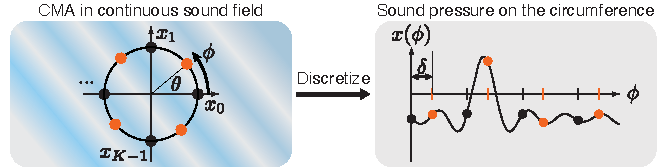
\includegraphics{figures/diagrams/sfi.pdf}
  \caption{%
    Concept of sound field interpolation on a CMA.
    The left figure depicts the CMA in a continuous sound field (six microphones in this example).
    Each black dot is a microphone at the reference position, and each gray dot is a microphone at the rotated position.
    Background colors indicate the sound pressure of a plane wave.
    The right side depicts the sound pressure along the circumference.
  }%
  \label{fig:sfi}
\end{figure}

Next, we formulate a sound field interpolation problem with the model above.
We define the $\Mic$-points spatial discrete Fourier transform (DFT) of $\sfcma _{\mic}$ and its inverse transform as
\begin{align}
  \dft _{\Src} [\sfcma _{\mic}] &= \sum _{\mic \in \SRC} \sfcma _{\mic} \twid ^{-\mic\src} \coloneqq \Sfcma _{\src},\\
  \dft _{\Src} ^{-1} [\Sfcma _{\src}] &= \frac{1}{\Mic} \sum _{\src \in \SRC} \Sfcma _{\src} \twid ^{\mic\src},%\\
  % \twid &= \exp \left(j\frac{2\pi}{\Mic}\right),
\end{align}
where $\twid \coloneqq \exp (j \frac{2\pi}{\Mic})$ is a twidle factor of $\Mic$-point DFT, $j$ is the imaginary unit,
and $\SRC$ is a index set defined as%{\small\todo{(和の範囲を次のようにとる理由…?)}}
\begin{align}
  \SRC &=
  \begin{cases}
    \left\{-\frac{\Src}{2} + 1, -\frac{\Src}{2} + 2, \dots, \frac{\Src}{2}\right\} & \text{($\Src$ is even)} \\
    \left\{-\frac{\Src - 1}{2}, -\frac{\Src - 1}{2} + 1, \dots, \frac{\Src - 1}{2}\right\} & \text{($\Src$ is odd)}
  \end{cases}
\end{align}
As is well known, the shift theorem of DFT, the following equation is satisfied for any integers $d$;
\begin{equation}
  \dft _{\Src} [\sfcma _{\mic + d}] = \Sfcma _{\src} \twid ^{d \src}.%
  \label{eq:sfi:shift:int}
\end{equation}
Although \eqref{eq:sfi:shift:int} does not hold strictly for real numbers, we assume that the following equation holds approximately for a real number $\rotSmpl$;
\begin{equation}
  \dft _{\Src} [\sfcma _{\mic + \rotSmpl}] = \Sfcma _{\src} \twid ^{\rotSmpl \src}.%
  \label{eq:sfi:shift:dft}
\end{equation}
From these assumptions, we have
\begin{align}
  \sfcma _{\mic + \rotSmpl} &= \dft _{\Src} ^{-1} \left[\Sfcma _{\src} \twid ^{\rotSmpl \src}\right], \\
                            &= \frac{1}{\Mic} \sum _{\src \in \SRC} \left(\Sfcma _{\src}\twid ^{\rotSmpl\src} \right) \twid ^{\mic\src}, \\
                            &= \frac{1}{\Mic} \sum _{\src \in \SRC} \left(\sum _{n=0} ^{\Mic - 1} \sfcma _{n} \twid ^{-n\src}\right) \left( \twid ^{(\rotSmpl + \mic)\src} \right), \\
                            &= \sum _{\dum = 0} ^{\Mic - 1} \sfcma _{\dum} \left( \frac{1}{\Mic} \sum _{\src \in \SRC} \twid ^{(\rotSmpl + \mic - \dum)\src} \right)
                            \coloneqq \sum _{\dum = 0} ^{\Mic - 1} \sfcma _{\dum} \rotmat _{\mic, \dum}(\rotSmpl) \label{eq:sfi:elem}.
\end{align}
The coefficient $\rotmat _{\mic,\dum}(\rotSmpl)$ is calculated as
\begin{align}
  \rotmat _{\mic,\dum}(\rotSpat)
  &=
    \begin{cases}
      \displaystyle\frac{\twid ^{- \rotIdx (\frac{\Mic}{2} - 1) }}{\Mic} \frac{1 - \twid ^{\rotIdx \Mic}}{1 - \twid ^{\rotIdx}}\\[1em]
      \displaystyle\frac{\twid ^{- \rotIdx \frac{\Src - 1}{2}}}{\Mic} \frac{1 - \twid ^{\rotIdx \Mic}}{1 - \twid ^{\rotIdx}}
    \end{cases}
  =
    \begin{cases}
      \displaystyle \frac{\sinc{(\rotIdx)}}{\sinc{\left(\rotIdx / \Mic\right)}} \twid ^{\frac{\rotIdx}{2}} & (\text{$\Mic$ is even}),\\[1em]
      \displaystyle \frac{\sinc{(\rotIdx)}}{\sinc{\left(\rotIdx / \Mic\right)}} & (\text{$\Mic$ is odd}),
    \end{cases}\label{eq:rot:sinc}
\end{align}
where and $\rotIdx =\rotSmpl + \mic - \dum; (\mic, \dum = 0, \dots, \Mic - 1)$ \cite{Wakabayashi:2023:ASLP}.
\eqref{eq:rot:sinc} is an alternative expression for (3) in \cite{Wakabayashi:2023:ASLP}.
See Section II of \cite{Wakabayashi:2023:ASLP} for the detailed derivation.

The above relationship also holds in the frequency domain.
Let us define the following vector:
\begin{align}
  \bm{\sfcma} &= \begin{bmatrix} \sfcma _{0} & \dots & \sfcma _{\Mic - 1} \end{bmatrix} ^{\top}, \\
  \bm{\sfcma} _{\rotSmpl} &= \begin{bmatrix} \sfcma _{0+\rotSmpl} & \dots & \sfcma _{(\Mic - 1)+\rotSmpl} \end{bmatrix} ^{\top}.
\end{align}
From \eqref{eq:sfi:elem}, we have
\begin{equation}
  \bm{\sfcma} _{\rotSmpl}
  =
  \begin{bmatrix}
    \rotmat _{0, 0}(\rotSpat) & \dots & \rotmat _{0, \Mic - 1}(\rotSpat) \\
    \vdots & \ddots & \vdots \\
    \rotmat _{\Mic - 1, 0}(\rotSpat) & \dots & \rotmat _{\Mic - 1, \Mic - 1}(\rotSpat)
  \end{bmatrix}
  \bm{\sfcma}
  \coloneqq
  \rotMat (\rotSpat) \bm{\sfcma},
  \label{eq:rotmat}
\end{equation}
where $\rotMat (\rotSpat) \in \C ^{\Mic\times\Mic}$ is \emph{rotation matrix}.
By definition, $\rotMat (\rotSpat)$ is obviously a unitary matrix; $\rotMat ^{-1} (\rotSpat) = \rotMat ^{\hermite} (\rotSpat)$.
Next, let $\bm{\Sfcma}$ be its DFT defined as $\begin{bmatrix} \Sfcma _{0} & \dots & \Sfcma _{\Mic - 1}\end{bmatrix} ^{\top} = \bm{F} \bm{\sfcma}$, where $\bm{F}$ is a $\Src$-points DFT matrix.
By using these expression, $\rotMat (\rotSpat)$ can be diagonarized as $\bm{F}^{\hermite} \rotMat (\rotSpat) \bm{F}$ since $\rotMat (\rotSpat)$ is a unitary matrix.
Therefore, the relationship between $\bm{\Sfcma}$ and $\bm{\Sfcma} _{\rotSmpl}$ can be expressed as $\bm{X} _{\rotSmpl} = \rotMat (\rotSpat) \bm{X}$,
because $\bm{\sfcma} _{\rotSmpl} = \bm{F}^{\hermite} \rotMat (\rotSpat) \bm{F} \bm{\sfcma}$.

In the STFT domain, we consider a situation where CMA is rotated of degree $\rotSpat _{\tframe}$ at time frame $\tframe$ and let $\refpos{\Obs} _{\ft}$ be the observed signal recorded without CMA rotation (\emph{reference position}).
By using the expression above, we assume that the observed signal with CMA rotation $\Obs _{\ft}$ is expressed as the following linear approximation:
\begin{equation}
  \refpos{\Obs} _{\ft} = \rotMat ^{-1} (\rotSpat _{\tframe}) \Obs _{\ft}.
\end{equation}
Note that $\rotSpat _{\tframe}$ must be known with another sensor, such as an angular acceleration sensor, or estimated from acoustic observation itself \cite{Lian:2021:APSIPA}.

\section{Proposed Method}\label{sec:proposed}


\subsection{SFI-based Online AuxIVA with Transformation of Latest Observation}
% TODO: 観測信号に対する音場補間,W/Vに対する変換との違いのイメージ図

% 本節では,CMAの回転に頑健なonline BSSを提案するために,BSSと文献1で提案されたSFIを組み合わせることを考える.
% 通常のOnline AuxIVAでは回転前後で分離行列を推定し直す必要がある.
% 前述したように,CMAの回転角度と回転時刻が得られていれば,SFIによってCMAの回転をキャンセルできため,分離行列を推定し直すことなく音源分離できる.
In the beamforming robust against the self-rotation proposed in \cite{Wakabayashi:2023:ASLP}, the signals observed by the CMA with angle $\theta_t$ are transformed frame by frame to what would have been observed at the reference position, namely at angle $\theta=0$, using SFI, and then the beamforming is applied to the transformed signals.

To make the OIVA robust against self-rotation, we first consider a similar approach to \cite{Wakabayashi:2023:ASLP} in this subsection.
In this method, we simply apply the transformation using SFI to the latest observation:
\begin{align}
  \refpos{\Obs} _{\ft} &\gets \rotMat ^{\hermite} (\rotSpat _{\tframe}) \Obs _{\ft},
  \label{eq:sfi:obs}
\end{align}
and the online update of the weighted covariance matrix $\cov _{\src,\ft}$ is performed by the transformed signal $\refpos{\Obs} _{\ft}$ such as
\begin{align}
  \cov _{\src,\ft}\gets \forget \cov _{\src,\ft[-1]} + (1 - \forget) \weight(\var _{\src,\tframe}) \refpos{\Obs} _{\ft} \refpos{\Obs} _{\ft} ^{\hermite}.
  \label{eq:cov:rot}
\end{align}
The demixing matrices $\Demix _{\ft}$ are estimated by using these weighted covariance matrices $\cov _{\src,\ft}$ in the OIVA manner. \Cref{alg:sfiva-o} summarizes OIVA using this approach.

Assuming that CMA rotates only once at a specific time frame $\tframe$, we analyze how the proposed method, as given in \cref{eq:cov:rot}, differs from the original formula in \cref{eq:cov}.
In \cref{eq:cov}, the value of $\cov _{\src,\ft}$ is updated online.
However, since the angles of CMA differ between time frames $\tframe - 1$ and $\tframe$, the blending of $\cov _{\src,\ft[-1]}$, which holds information before the rotation, and $\Obs _{\ft}$, which holds information after the rotation, leads to an inaccurate estimation of the demixing matrix $\Demix _{\ft}$.
If CMA does not rotate further after time frame $\tframe$,
the observation information before the rotation is gradually diminished, and
$\cov _{\src,\ft}$ and $\Demix _{\ft}$ are expected to slowly converge to their values
associated with the post-rotation position of CMA.
However, this convergence is expected to take time.
On the contrary, in \cref{eq:cov:rot}, all observed signals are translated into observation at the reference position.
Thus, even if CMA rotates at time frame $\tframe$, there is no substantial discrepancy between $\cov _{\src,\ft[-1]}$ and $\refpos{\Obs} _{\ft}$, and the influence of rotation on the estimation of the demixing matrix $\Demix _{\ft}$ is expected to be much reduced.

Note that  the separated signals obtained by this approach are the source images at the reference microphone of CMA with the reference angle, regardless of the CMA rotation.
%As a result, the source image at the rotated position cannot be obtained,
It causes problems in some practical applications.
%BSS in augmented reality space using a head-mounted display needs to be processed so that the sound can be heard from the position of the source image after rotation.
For example, in hearing aid applications or virtual/augmented reality (VR/AR) applications with a head-mounted display, it is desired to present a separated signal with the source localization sensation.
For this purpose, we need to estimate the source images on the reference microphone of the CMA rotated together with a head.

\begin{algorithm}{SFI-based Online AuxIVA using Transformation of Latest Observation (\SFIIVAo)}{sfiva-o}
  \textbf{Input:} ${\{\Obs _{\ft}\}} _{\ft}$, ${\{\Demix _{\freq,0}\}} _{\freq}$, ${\{\cov _{\src,\freq,0}\}} _{\src,\freq}$, $\forget$, ${\{\rotSpat _{\tframe}\}} _{\tframe}$ \\
  \textbf{Output:} ${\{\Est _{\ft}\}} _{\ft}$
  \begin{pseudo}
    % for $\tframe = 1,\, \dots,\, \rotFra - 1$ \ct{Demixing matrix update before rotation} \\+
    %   \nf{Run \cref{alg:iva}} \\-
    for $\tframe = 1,\, \dots,\, \Tframe$ \\+
      for $\freq = 1, \dots, \Freq$ \\+
        $\refpos{\Obs} _{\ft} \gets \rotMat ^{\hermite} (\rotSpat _{\tframe}) \Obs _{\ft}$ \ct{\eqref{eq:sfi:obs}} \\
        {$\Demix _{\ft}$} $\gets$ $\Demix _{\ft[-1]}$ \\-
      for $\itr = 1,\, \dots,\, \Itr$ \\+
        for $\src = 1,\, \dots,\, \Src$ \\+
          {$\var _{\src,\tframe}$} $\gets$ $\sqrt{\sum _{\freq = 1} ^{\Freq} \abs{\demix _{\src,\ft} ^{\hermite} \refpos{\Obs} _{\ft}} ^2}$ \ct{\eqref{eq:var}} \\
          for $\freq = 1, \dots, \Freq$ \\+
            {$\cov _{\src,\ft}    $} $\gets$ $\forget \cov _{\src,\ft[-1]} + (1 - \forget) \weight(\var _{\src,\tframe}) \refpos{\Obs} _{\ft} \refpos{\Obs} _{\ft} ^{\hermite}$ \ct{\eqref{eq:cov:rot}} \\
            {$\demix _{\src,\ft}$} $\gets$ $\left(\Demix _{\ft} \cov _{\src,\ft}\right) ^{-1} \eye _{\src}$ \ct{\eqref{eq:ip:proj}} \\
            {$\demix _{\src,\ft}$} $\gets$ $\frac{\demix _{\src,\ft}}{\sqrt{\demix _{\src,\ft} ^{\hermite} \cov _{\src,\ft} \demix _{\src,\ft}}}$ \ct{\eqref{eq:ip:norm}} \\---

      % \nf{$
      %   \begin{bsmallmatrix}
      %     \str _{1,1,\ft} & \dots & \str _{1,\Src,\ft} \\
      %     \vdots & \ddots & \vdots \\
      %     \str _{\Src,1,\ft} & \dots & \str _{\Src,\Src,\ft}
      %   \end{bsmallmatrix} \gets \Demix _{\ft} ^{-1}$} \ct{$\forall \freq$} \\
      % \nf{$\proj{\Demix} _{\ft} \gets \diag\left(\str _{1,1,\ft} \; \str _{1,2,\ft}\; \dots \; \str _{1,\Src,\ft}\right) \Demix _{\ft}$} \ct{\eqref{eq:pb:w}}\\
      for $\freq = 1, \dots, \Freq$ \\+
        \nf{$\proj{\Demix} _{\ft} \gets \diag\left(\eye _{1} ^{\top} \Demix _{\ft} ^{-1} \right) \Demix _{\ft}$} \ct{\eqref{eq:pb:w}}\\
        {$\Est _{\ft}$} $\gets$ $\proj{\Demix }_{\ft} \refpos{\Obs} _{\ft}$ \ct{\eqref{eq:pb:y}}
  \end{pseudo}
\end{algorithm}

\subsection{SFI-based Online AuxIVA with Transformation of Pre-update Demixing and Weighted Covariance Matrices}\label{subsec:proposed:sfiivam}

% 前節の問題を解決するために,マイクの位置を保ったままCMA回転に頑健なonline BSSを提案する.
% 観測信号のかわりにパラメータを変換することで,CMAが回転した後の位置におけるsource imageを得る手順を示す.
% まず,簡単のために,時不変な環境におけるパラメータ変換を議論する.
% 角度$\rotSpat$回転したCMAで録音された観測信号が,次の関係を厳密に満たしていると仮定する:

In this subsection, we propose another online BSS which is robust against CMA rotation and outputs the source image at the latest microphone position.
As discussed in the previous section, the mismatch between $\cov _{\src,\ft[-1]}$ and $\Obs _{\ft}$ causes a problem.
In the previous approach, we transform $\Obs _{\ft}$ to what it should be at the reference position of CMA.
In this subsection, we consider another approach: transforming $\cov _{\src,\ft[-1]}$ to what it should be at the latest position of CMA.

%We present a procedure to obtain the source image at the position after the CMA rotation by transforming the parameters instead of the observed signal.
First, we discuss the parameter transformation in a \emph{time-invariant} case for simplicity.
In this case, demixing matrices $\Demix _{\freq}$ and weighted covariance matrices $\cov _{\src,\freq}$ are independent on time frame $\tframe$.
Let $\Obs _{\ft}$ and $\refpos{\Obs}_{\ft}$ are observations if the angle of CMA is fixed at $\rotSpat _1$ and $\rotSpat _2$, respectively.
If the approximation of SFI is satisfied, $\Obs _{\ft}$ and $\refpos{\Obs} _{\ft}$ hold the following relation:
\begin{equation}
  \refpos{\Obs} _{\ft} = \rotMat (\Delta\rotSpat)\Obs _{\ft},
\end{equation}
where $\Delta\rotSpat = \rotSpat _2 - \rotSpat _1$.
From this, we have the estimated signal $\Est _{\ft}$ as:
\begin{align}
  \Est _{\ft} &= \Demix _{\freq} \Obs _{\ft}, \\
              &= \Demix _{\freq} \rotMat ^{\hermite} (\Delta\rotSpat) \refpos{\Obs} _{\ft} \coloneqq \refpos{\Demix} _{\freq} \refpos{\Obs} _{\ft}, \label{eq:rt:demix:batch}
\end{align}
% $\refpos{\Demix} _{\freq}$は,reference positionにおける観測信号を用いて推定された時不変な分離行列とみなせる.
% 同様に,$\refpos{\Obs} _{\ft}$を用いて推定された時不変な共分散行列 $\refpos{\cov} _{\src,\freq}$ は次で計算される:
where $\Demix_{\freq}$ and $\refpos{\Demix} _{\freq}$ are time-invariant demixing matrices
for $\Obs _{\ft}$ and $\refpos{\Obs} _{\ft}$, respectively.
Therefore,
\begin{align}
  \refpos{\Demix} _{\freq} = \Demix _{\freq} \rotMat ^{\hermite} (\Delta\rotSpat). \label{eq:demix:refpos}
\end{align}
Similarly, the time-invariant weighted covariance matrix $\cov_{\src,\freq}$ estimated using $\Obs_{\ft}$ is calculated by:
\begin{equation}
  \cov _{\src,\freq} = \expct  _{\tframe} \left[\weight (\var _{\src,\tframe}) \Obs _{\ft} \Obs _{\ft} ^{\hermite}\right],
  % \weight (\var _{\src,\tframe}) &= \frac{1}{\Freq} \sum _{\freq = 1} ^{\Freq} \lvert \refpos{\demix} _{\src,\freq} ^{\hermite} \refpos{\Obs} _{\ft} \rvert ^2,
\end{equation}
% ただし,$\expct _{\tframe}\left[\bm{A} _{\tframe}\right]$は,ある確率変数行列$\bm{A}_{\tframe}$の時間フレーム$\tframe$に対する期待値演算である.
% $\Obs _{\ft}$の共分散行列${\cov} _{\src,\freq}$を,$\refpos{\cov} _{\src,\freq}$を用いて表すことを考える.
% $\refpos{\Demix} _{\freq} = \Demix _{\freq} \rotMat (\rotSpat)$より,その各行ベクトルは$\refpos{\demix} _{\src,\freq} ^{\hermite} = \demix _{\src,\freq} ^{\hermite} \rotMat (\rotSpat)$であるので,
% 重み関数$\weight(\var _{\src,\tframe})$は,
where $\expct _{\tframe}\left[\bm{A} _{\tframe}\right]$ is the expectation operation for a random variable matrix $\bm{A}_{\tframe}$ with respect to time frame $\tframe$.
We rewrite the weighted covariance matrix ${\cov} _{\src,\freq}$ of $\Obs _{\ft}$ using $\refpos{\cov} _{\src,\freq}$ as:
\begin{align}
  \refpos{\cov} _{\src,\freq} &= \expct  _{\tframe} \left[\weight (\var _{\src,\tframe}) \refpos{\Obs} _{\ft} \refpos{\Obs} _{\ft} ^{\hermite}\right], \\
                     &= \expct  _{\tframe} \left[\weight (\var _{\src,\tframe}) \rotMat (\Delta\rotSpat) {\Obs} _{\ft} {\Obs} _{\ft} ^{\hermite} \rotMat ^{\hermite} (\Delta\rotSpat)\right], \\
                     &= \rotMat (\Delta\rotSpat)\; \expct  _{\tframe} \left[\weight (\var _{\src,\tframe}) {\Obs} _{\ft} {\Obs} _{\ft} ^{\hermite} \right] \rotMat ^{\hermite} (\Delta\rotSpat), \\
                     &= \rotMat (\Delta\rotSpat) {\cov} _{\src,\freq} \rotMat ^{\hermite} (\Delta\rotSpat). \label{eq:cov:refpos:batch}
\end{align}
% したがって,CMAの回転角度$\rotSpat$とその時刻$\rotFra$を知っていれば,その時刻において\eqref{eq:rt:demix:batch}, \eqref{eq:rt:cov:batch}の変換を行うことで前節と同じ結果を得ることができる.
%Therefore, if we know the rotation angle $\rotSpat$ and its time frame $\rotFra$, we can get the same result as the previous subsection by performing the transformations \eqref{eq:rt:demix:batch} and \eqref{eq:rt:cov:batch}.

% 以上の結果の近似として,オンラインAuxIVAにおいては次の式を用いて,CMA回転時刻においてパラメータを変換する:
Although $\cov _{\src,\ft}$ and $\Demix _{\ft}$ are estimated online in OIVA,
we use these variable transformations written in \eqref{eq:demix:refpos} and \eqref{eq:cov:refpos:batch} as a pre-processing of their update to compensate of the CMA rotation such as:
%For OIVA, we perform the following transformation at the rotation time $\rotFra$ as an approximation of the results above:
\begin{align}
  \refpos{\Demix} _{\ft[-1]} &\gets \Demix _{\ft[-1]} \rotMat ^{\hermite} (\Delta \rotSpat _{\tframe}), \label{eq:sfiiva:demix} \\
  \refpos{\cov} _{\src,\ft[-1]} &\gets \rotMat (\Delta\rotSpat _{\tframe}) \cov _{\src,\ft[-1]} \rotMat ^{\hermite} (\Delta\rotSpat _{\tframe}), \label{eq:sfiiva:cov}
\end{align}
where $\Delta\rotSpat _{\tframe} = \rotSpat _{\tframe} - \rotSpat _{\tframe - 1}$.
% この手法は観測信号はマイクが回転した信号を変換せずに扱うことができるため,回転後の位置における音像が推定される.
% さらに,前節の観測信号に対して音場補間する手法とは異なり,回転後の毎フレームに対して変換が必要なく,回転した時間フレーム時点の1回だけ変換を行えばよい.
The whole algorithm is summarized as \cref{alg:sfiva-m}.
This method preserves the observation as-is and transforms the intermediate variables as $\Demix _{\ft[-1]}$ and $\cov _{\src,\ft[-1]}$ instead, the source image at the latest CMA position can be estimated, which is an advantage of this algorithm.
Furthermore, the angle of CMA is supposed to be measured by integrating angular accelerometers, which can introduce bias errors.
In this case, the method described in the previous subsection continues to have errors in the transformation of the observations to those at the reference position.
On the other hand, in the method described in this subsection, the error included in the transformation of $\Demix _{\ft}$ and $\cov _{\src,\ft}$ should disappear with online updates.
This is another advantage of this approach. We will show this in an experiment to be described later.

%This method can handle the observed signal without transforming the observed signal after the CMA rotation, so the source image at the post-rotated position is estimated.
%Furthermore, unlike the method of SFI for the observation signal in the previous subsection, no transformation is required for every single frame after rotation, and only one transformation at the time of the rotated time frame is needed.
%\todo{%
%  \paragraph{TODO}
%  \begin{itemize}
%    \item 回転角度は時間インデクスを含めて一般的に$\rotSpat _{\tframe}$で表し,4.2の時不変の話を出さずに書きたい
%    \begin{itemize}
%      \item[$\Rightarrow$] \eqref{eq:rt:cov:batch}の変換をどう正当化するか?
%      \item[$\Rightarrow$] SFIIVA-Mの利点として当初主張していた「回転した瞬間だけ計算すればよい」が言えなくなる,むしろ計算量が大きくなってしまう…
%      \item[$\Rightarrow$] 現状の実験結果は回転1回なので,5章で結局,回転角度はある時刻$\rotFra$で一回だけ回転という話に戻す必要がある
%    \end{itemize}
%  \item 角度の測定誤差があるときの利点
%    \begin{itemize}
%      \item SFIIVA-Oは誤差が蓄積する
%      \item SFIIVA-Mはオンライン更新で忘れていくので,推定角度が間違っていても収束するはず
%        \begin{itemize}
%          \item 大きなメリットといえる (by 若林先生),わかりやすく主張しておきたい
%        \end{itemize}
%    \end{itemize}
%\end{itemize}
%}

\begin{algorithm}{SFI-based Online AuxIVA with Transformation of Pre-update Demixing and Weighted Covariance Matrices (\SFIIVAm)}{sfiva-m}
  \textbf{Input:} ${\{\Obs _{\ft}\}} _{\ft}$, ${\{\Demix _{\freq,0}\}} _{\freq}$, ${\{\cov _{\src,\freq,0}\}} _{\src,\freq}$, $\forget$, ${\{\rotSpat _{\tframe}\}} _{\tframe}$ \\
  \textbf{Output:} ${\{\Est _{\ft}\}} _{\ft}$
  \begin{pseudo}

    for $\tframe = 1,\, \dots,\, \Tframe$ \\+
      $\varDelta \rotSpat _{\tframe} \gets \rotSpat _{\tframe} - \rotSpat _{\tframe - 1}$ \\
      for $\freq = 1, \dots, \Freq$ \\+
        {$\Demix _{\freq,\tframe}$} $\gets$ $\Demix _{\freq,\tframe - 1} \rotMat ^{\hermite} (\varDelta\rotSpat _{\tframe})$ \ct{\eqref{eq:sfiiva:demix}} \\
        for $\src = 1,\, \dots,\, \Src$ \\+
          {$\refpos{\cov} _{\src,\ft[-1]}$} $\gets$ $\rotMat (\varDelta\rotSpat _{\tframe}) \cov _{\src,\ft[-1]} \rotMat ^{\hermite} (\varDelta \rotSpat _{\tframe})$ \ct{\eqref{eq:sfiiva:cov}} \\--
      for $\itr = 1,\, \dots,\, \Itr$ \\+
        for $\src = 1,\, \dots,\, \Src$ \\+
          {$\var _{\src,\tframe}$} $\gets$ $\sqrt{\sum _{\freq = 1} ^{\Freq} \abs{\demix _{\src,\ft} ^{\hermite} \Obs _{\ft}} ^2}$ \ct{\eqref{eq:var}} \\
          for $\freq = 1, \dots, \Freq$ \\+
            {$\cov _{\src,\ft}    $} $\gets$ $\forget \refpos{\cov} _{\src,\ft[-1]} + (1 - \forget) \weight(\var _{\src,\tframe}) \Obs _{\ft} \Obs _{\ft} ^{\hermite}$ \\
            {$\demix _{\src,\ft}$} $\gets$ $\left(\Demix _{\ft} \cov _{\src,\ft}\right) ^{-1} \eye _{\src}$ \ct{\eqref{eq:ip:proj}} \\
            {$\demix _{\src,\ft}$} $\gets$ $\frac{\demix _{\src,\ft}}{\sqrt{\demix _{\src,\ft} ^{\hermite} \cov _{\src,\ft} \demix _{\src,\ft}}}$ \ct{\eqref{eq:ip:norm}} \\---

      for $\freq = 1, \dots, \Freq$ \\+
        \nf{$\proj{\Demix} _{\ft} \gets \diag\left(\eye _{1} ^{\top} \Demix _{\ft} ^{-1} \right) \Demix _{\ft}$} \ct{\eqref{eq:pb:w}}\\
        {$\Est _{\ft}$} $\gets$ $\proj{\Demix }_{\ft} \Obs _{\ft}$ \ct{\eqref{eq:pb:y}}
  \end{pseudo}
\end{algorithm}

\section{Experimental Validation}\label{sec:experiment}
% Although OIVA can track slow microphone movements, its convergence performance highly depends on the forgetting factor.
% Furthermore, ICA-based BSS methods do not change the results even if the observed signals are ``remixed.''
% For example, the same output is obtained by inputting the 2-channel observed signals $x_1$ and $x_2$ as $x_1 + x_2$ and $x_1 - x_2$.
% Since the transformation of the observed signals by the SFI can also be interpreted as a kind of ``remixing,''
% the separation performance is expected to remain the same regardless of whether or not the SFI is performed before or after the CMA rotation.
% However, it has been reported that SFI improves the separation performance \cite{Nakashima:2022:ASJ:A}.
In this section, we experimentally confirm how much SFI contributes to BSS and discuss the difference in the location of the source image due to the SFI.
Henceforth, we assume that CMA was instantaneously rotated at an angle $\rotSpat$ at time frame $\rotFra$.

\subsection{Setup}

Simulation experiments with large random synthesized datasets were conducted to evaluate the performance of BSS under a situation where CMA rotates.
The datasets consisted of 100 samples, and each sample simulated observed signals with five source signals with 5-channel CMA using the image source method \cite{Allen:1979:JASA}.
As the source signal, we used the speech signals of five speakers (\texttt{jvs001}, \texttt{jvs002,} $\hdots$, \texttt{jvs005}) from the JVS dataset \cite{Takamichi:2019:arxiv}.
In this experiment, the utterances included in \texttt{parallel100} were randomly concatenated for each speaker.
The length was \SI{60}{\second}, and the sampling frequency was resampled from \SI{24}{\kilo\hertz} to \SI{16}{\kilo\hertz}.
The reverberation time was approximately \SI{100}{\milli\second}.
A CMA with $\Src = 5$ channels and a radius of \SI{2}{\centi\metre} was placed in the center of the room.
Each source was randomly placed at least \SI{1}{\metre} from the center of the CMA and within an angle ranging from $\frac{360}{\Src} \src$ to $\frac{360\si{\degree}}{\Src} (\src - 1) + \frac{180\si{\degree}}{\Src}\; (\src = 1, \dots, \Src)$.
%   0,  36
%  72, 108
% 144, 180
% 216, 252
% 288, 324
\Cref{fig:layout:exp} illustrates the range of the sources' placement and its example.
To simulate the instant rotation of the CMA, the source images were generated when the CMA was rotated \SI{40}{\degree} counter-clockwise from the horizontal axis and was stitched together in the 0--30\si{\second} and 30--60\si{\second} intervals, respectively.
Note that the rotation angle and time are given oracle-manner.
STFT was performed on the observed signals with a frame length of 4096 points, a shift length of 2048 points, and a Hamming window.
The scale of the output signal was restored by the back-projection shown in \cref{alg:iva}, with the reference microphone as microphone 1.
The separation performance was evaluated by the scale-invariant signal-to-distortion ratio (SI-SDR) \cite{LeRoux:2019:ICASSP} and its improvement (SI-SDR improvements; SI-SDRi).
The reference signal for the SI-SDR was the source image recorded with a rotated CMA.
\begin{figure}[t]
  \centering
  \begin{minipage}[t]{.32\linewidth}
    \centering
    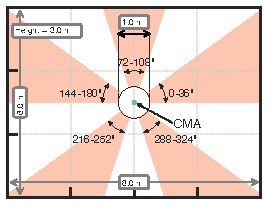
\includegraphics[width=\columnwidth]{figures/room_layout_range.pdf}
    \subcaption{Sources are randomly placed in the orange shaded area.}%
    \label{fig:layout:range}
  \end{minipage}
  \begin{minipage}[t]{.32\linewidth}
    \centering
    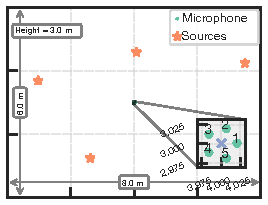
\includegraphics[width=\columnwidth]{figures/room_layout_000.pdf}
    \subcaption{Example before rotation.}%
    \label{fig:layout:ref}
  \end{minipage}
  \begin{minipage}[t]{.32\linewidth}
    \centering
    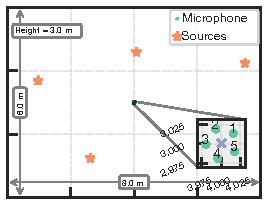
\includegraphics[width=\columnwidth]{figures/room_layout_040.pdf}
    \subcaption{Example after rotation.}%
    \label{fig:layout:rot}
  \end{minipage}
  \caption{Room layout.}%
  \label{fig:layout:exp}
\end{figure}

The initial values for demixing and weighted covariance matrices were
$\Demix _{\freq,0} = \Eye\; (\forall \freq)$, $\cov _{\src,\freq,0} = 10^{-3} \times \Eye\; (\forall \src, \freq)$, respectively, where $\Eye$ is the $\Src$-dimensional identity matrix.
We set the number of iterations in each time frame in \cref{alg:iva} $\Itr$ to 5.
We ran experiments with varying forgetting factors $\forget = 0.9, 0.95, 0.98, 0.99$, which were chosen so that the approximate number of frames $\frac{1}{1 - \forget} = 10, 20, 50, 100$.
To increase numerous stability for the implementation of OIVA,
we applied the following ad-hoc normalization $\cov _{\src,\ft} \gets \cov _{\src,\ft} + 10 ^{-3} \times \Eye$ after updates by \eqref{eq:cov}.
We compared the following four methods:
\begin{description}
  \item[\NaiveIVA] OIVA described in \cref{subsec:oiva} as a baseline.
  \item[\ResetIVA] Re-initialize weighted covariance and demixing matrices when the CMA was rotated:
      $\Demix _{\freq,\rotFra - 1} \gets \Eye, \; \cov _{\src,\freq,\rotFra - 1} \gets \varepsilon \Eye.$
  \item[\SFIIVAo] Apply SFI for observed signals after the CMA rotation CMA frame by frame. (See \Cref{alg:sfiva-o}.)
    % \\ $\Obs _{\ft} = \rotMat ^{\hermite} (\rotSpat _{\tframe}) \rot{\Obs} _{\ft}$
  \item[\SFIIVAm] Apply parameter transformation for weighted covariance and demixing matrices after CMA rotation.  (See \Cref{alg:sfiva-m}.)
    % \\ $\rot{\Demix} _{\ft} \gets \Demix _{\ft} \rotMat ^{\hermite} (\rotSpat _{\tframe})$,\; $\rot{\cov} _{\src,\ft} \gets \rotMat (\rotSpat _{\tframe}) \cov _{\src,\ft} \rotMat ^{\hermite} (\rotSpat _{\tframe})$
\end{description}

\subsection{Source Separation Performance}

\Cref{fig:plot:line} shows the SI-SDRi every \SI{1}{\second} averaged over samples and channels.
\Cref{fig:plot:box} shows the SI-SDRi averaged over samples and channels immediately after and after a sufficient time has elapsed of CMA rotation.
Overall, \NaiveIVA{} and \ResetIVA{} showed a performance drop immediately after the CMA rotation and improved again with time.
\ResetIVA{} has the lowest performance before CMA rotation among all forgetting factors, which worsens as the forgetting factor approaches 1.
In contrast, the proposed \SFIIVAm{} and \SFIIVAo{} methods performed better performance immediately after the CMA rotation than the others.
Comparing \SFIIVAm{} and \SFIIVAo{}, \SFIIVAm{} performed slightly better.
This result may be because \SFIIVAo{} estimates the source image at the reference microphone, while the reference signal for SI-SDR evaluation was the source image at the reference position.
\begin{figure}[t]
  \centering
  \begin{minipage}[t]{.45\textwidth}
    \centering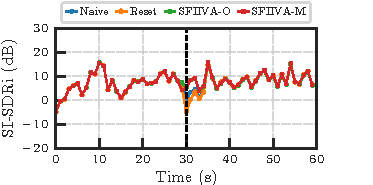
\includegraphics{figures/plots/online/line_900.pdf}\subcaption{$\forget = 0.9  $}\label{fig:plot:line:900}
  \end{minipage}
  \begin{minipage}[t]{.45\textwidth}
    \centering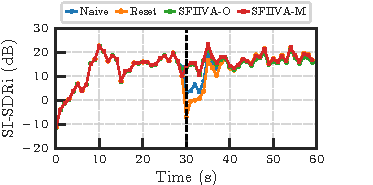
\includegraphics{figures/plots/online/line_950.pdf}\subcaption{$\forget = 0.95 $}\label{fig:plot:line:950}
  \end{minipage}

  \begin{minipage}[t]{.45\textwidth}
    \centering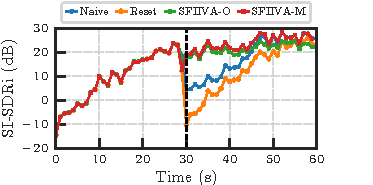
\includegraphics{figures/plots/online/line_980.pdf}\subcaption{$\forget = 0.98 $}\label{fig:plot:line:980}
  \end{minipage}
  \begin{minipage}[t]{.45\textwidth}
    \centering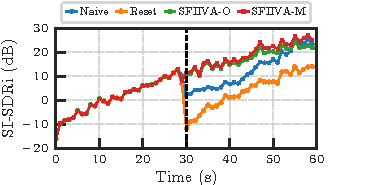
\includegraphics{figures/plots/online/line_990.pdf}\subcaption{$\forget = 0.99 $}\label{fig:plot:line:990}
  \end{minipage}
  \caption{SI-SDR improvements (SI-SDRi) every \SI{1}{\second}}%
  \label{fig:plot:line}
\end{figure}

\begin{figure}[t]
  \centering
  \begin{minipage}[t]{.45\textwidth}
    \centering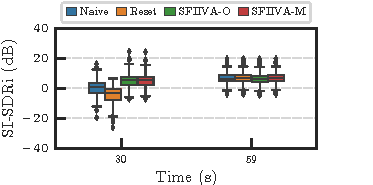
\includegraphics{figures/plots/online/box_900.pdf}\subcaption{$\forget = 0.9  $}\label{fig:plot:box:900}
  \end{minipage}
  \begin{minipage}[t]{.45\textwidth}
    \centering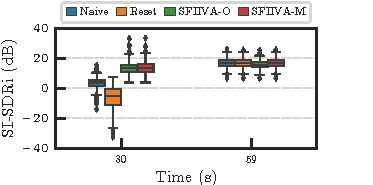
\includegraphics{figures/plots/online/box_950.pdf}\subcaption{$\forget = 0.95 $}\label{fig:plot:box:950}
  \end{minipage}

  \begin{minipage}[t]{.45\textwidth}
    \centering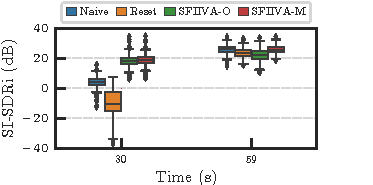
\includegraphics{figures/plots/online/box_980.pdf}\subcaption{$\forget = 0.98 $}\label{fig:plot:box:980}
  \end{minipage}
  \begin{minipage}[t]{.45\textwidth}
    \centering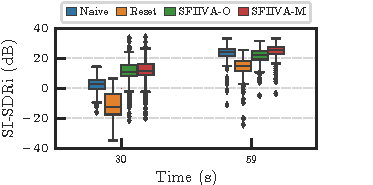
\includegraphics{figures/plots/online/box_990.pdf}\subcaption{$\forget = 0.99 $}\label{fig:plot:box:990}
  \end{minipage}
  \caption{Box plot of SI-SDR improvements (SI-SDRi) immediately after and after a sufficient time has elapsed of CMA rotation.}%
  \label{fig:plot:box}
\end{figure}

\subsection{Robustness against Estimation Error}

To check the robustness against errors in measuring the angle of CMA rotation, we compared results when the measured angles used for \SFIIVAo{} and \SFIIVAm{} differed from the true angle.
As discussed in \cref{subsec:proposed:sfiivam}, we expected errors to accumulate when there is an error in the measured angle since \SFIIVAo{} transforms the observed signal every frame.
In contrast, \SFIIVAm{} performs the transformation only at the CMA rotation, so the effect of the measuring error should decrease with time.

\Cref{tab:sdr} shows the averaged over samples and channels immediately after and after a sufficient time has elapsed of CMA rotation with a measuring error.
The forgetting factor $\forget$ was fixed to $0.98$ in this experiment.
As expected, the SI-SDRi of both methods dropped by about \SI{8}{\decibel} at \SI{30}{\second} immediately after the CMA rotation, when the measured angle was \SI{60}{\degree} which is different from the true angle of \SI{40}{\degree}.
On the other hand, comparing the performance at \SI{59}{\second}, sufficiently after the CMA rotation, the performance of \SFIIVAm{} was about \SI{5}{\decibel} higher than that of \SFIIVAo{}.
\begin{table}[t]
  \caption{%
    Average SI-SDRi (dB) immediately after and after a sufficient time has elapsed of CMA rotation.
    The length of simulated speech signals is \SI{60}{\second} long, and CMA was instantaneously rotated at \SI{30}{\second}.
    True accurate measurement of CMA rotation was \SI{40}{\degree} and inaccurate measurement was \SI{60}{\degree}.
    Forgetting factor $\forget = 0.98$.
  }%
  \label{tab:sdr}
  \centering
  \sisetup{%
    table-format=2.2,
    table-alignment-mode=format,
    table-auto-round=true,
    detect-weight=true,
  }
  \footnotesize
  \begin{minipage}[t]{.45\linewidth}
    \centering
    \subcaption{Accurate measurement.}%
    \label{tab:sdr:98}
    \begin{tabular}{lSS}
      \toprule
        Method   & \multicolumn{2}{c}{Time (s)} \\ \cmidrule{2-3}
                 &       {30} &       {59} \\
      \midrule
        SFIIVA-O &  17.988841 &  22.130434 \\ \rowcolor[gray]{0.8}
        SFIIVA-M &  18.796094 & \bfseries  25.623199 \\
      \bottomrule
    \end{tabular}
  \end{minipage}
  \hspace{.05\linewidth}
  \begin{minipage}[t]{.45\linewidth}
    \centering
    \subcaption{Inaccurate measurement.}%
    \label{tab:sdr:98}
    \begin{tabular}{lSS}
      \toprule
        Method   & \multicolumn{2}{c}{Time (s)} \\ \cmidrule{2-3}
                 &       {30} &       {59} \\
      \midrule
        SFIIVA-O &   9.922167 &  20.262950 \\ \rowcolor[gray]{0.8}
        SFIIVA-M &   9.980653 &  \bfseries 25.626287 \\
      \bottomrule
    \end{tabular}
  \end{minipage}
\end{table}

\subsection{Difference of Beam Patterns}

In this subsection, we picked one example to focus on the difference between two proposed methods \SFIIVAo{} and \SFIIVAo{}.
\Cref{fig:plot:beam} shows the beam patterns of demixing matrices calculated by each method.
\Cref{fig:plot:bp:ref} is the result calculated before rotation.
\Cref{fig:plot:bp:sfiivao} and \cref{fig:plot:bp:sfiivam} are the results with demixing matrices respectively calculated with \SFIIVAm{} and \SFIIVAo{} after rotation.
Dark regions in each plot represent nulls in that direction.
In the case of BSS, the desired result is that the direction of the estimated source is brighter, and the others are darker.
As shown in \cref{fig:plot:beam}, the results of \cref{fig:plot:bp:ref} and \cref{fig:plot:bp:sfiivao} were similar to each other, and only \cref{fig:plot:bp:sfiivam} was different from the others.
The dark areas of \cref{fig:plot:bp:ref} and \cref{fig:plot:bp:sfiivao} were nearly at the desired directions since \SFIIVAo{} approximately canceled the rotation of CMA and thus updated demixing matrices in the same direction even after the rotation.
For \SFIIVAm{}, the bright areas should be in the direction viewed from the position after the rotation, i.e., \SI{40}{\degree} less anti-clockwise than the previous result in this case.
The result in \cref{fig:plot:bp:sfiivam} gave the expected direction after the CMA rotation.
\begin{figure}[t]
  \centering
  \begin{minipage}[t]{\linewidth}
    \centering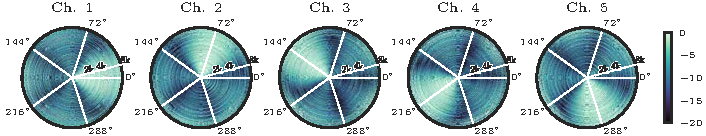
\includegraphics{figures/plots/beam-pattern/sfiiva-cov_ref.pdf}\subcaption{Before rotation.}\label{fig:plot:bp:ref}
  \end{minipage}
  \begin{minipage}[t]{\linewidth}
    \centering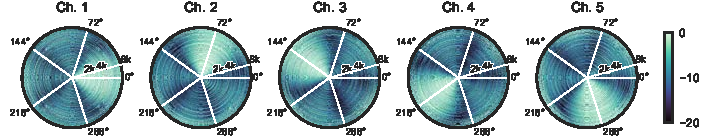
\includegraphics{figures/plots/beam-pattern/sfiiva-obs_rot.pdf}\subcaption{\SFIIVAo{} after rotation.}\label{fig:plot:bp:sfiivao}
  \end{minipage}
  \begin{minipage}[t]{\linewidth}
    \centering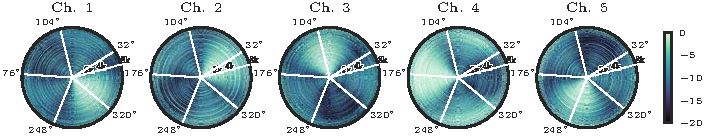
\includegraphics{figures/plots/beam-pattern/sfiiva-cov_rot.pdf}\subcaption{\SFIIVAm{} after rotation.}\label{fig:plot:bp:sfiivam}
  \end{minipage}
  \caption{%
    Beam patterns of demixing matrices.
    Five plots are the beam patterns of the frequency-wise demixing matrices calculated by each method.
    The radial direction of each plot represents the frequency, and the tangential direction represents the angle from the center of the CMA.
    The light and dark colors represent the gain in decibels.
    The five white lines in each plot represent the true direction of the source signal.
  }%
  \label{fig:plot:beam}
\end{figure}

\section{Conclusion}\label{sec:conclusion}
% 本研究では,円状等間隔マイクロホンアレイにおける音場補間をブラインド音源分離に応用した.
% 我々は2つの新しい手法を提案した;1つ目は音場補間とOIVAとの単純に組み合わせた手法,2つ目はパラメータ変換に基づく実用的な手法である.
% シミュレーション実験により,音場補間が円状等間隔マイクロホンアレイの回転に対するOIVAの頑健性を改善させたことを確認した.
% 今後は本手法の自己回転角度推定 \cite{Lian:2021:APSIPA} との組み合わせや,実時間処理への拡張などに取り組む.
In this study, sound field interpolation (SFI) for an equally spaced circular microphone array (CMA) was applied to online auxiliary-function-based independent vector analysis (OIVA).
We have proposed two new methods; the first is a simple combination of SFI and OIVA, and the second is a practical method based on parameter transformations.
Simulation experiments have confirmed that SFI improved the robustness of OIVA against the rotation of CMA.
Future work includes combining this method with self-rotation angle estimation \cite{Lian:2021:APSIPA} and extending it to real-time processing.

\section*{Biographies}

\noindent\normalsize\textbf{Taishi Nakashima}
received his B.E. in Engineering from Osaka University, Osaka, Japan, in 2019 and his M.S. in Informatics from Tokyo Metropolitan University, Tokyo, Japan, in 2021.
He is pursuing a Ph.D. at Tokyo Metropolitan University and has received the JSPS Research Fellowship (DC1) from April 2021.
He is an esteemed Student Member of the Acoustical Society of Japan (ASJ) and the IEEE Signal Processing Society (SPS).
He received the 24th Best Student Presentation Award of ASJ, the 16th IEEE SPS Japan Student Conference Paper Award in 2022, and the Top 3\% Recognition at ICASSP 2023.
His research interests primarily focus on blind source separation and acoustic signal processing.
\\

\noindent\normalsize\textbf{Yukoh Wakabayashi}
received the B.E. and M.E. degrees from Osaka University, Osaka, Japan, in 2008 and 2010, respectively, and Ph.D. degree from Ritsumeikan University, Shiga, Japan, in 2017.
He joined Rohm, Inc., Kyoto, Japan, in 2010, and was an assistant researcher with Kyoto University from 2012 to 2014.
He was a recipient of the JSPS Research Fellowship for Young Scientists DC2 from 2016 to 2017.
He was an affiliate assistant professor with Ritsumeikan University from 2018 to 2020.
He is currently an assistant professor with the Department of Computer Science and Engineering, Toyohashi University of Technology, Aichi, Japan, and the Faculty of Systems Design, Tokyo Metropolitan University, Tokyo, Japan.
His research interests include acoustic signal processing, speech phase processing, array signal processing, and speaker diarization.
He is a member of the Institute of Electrical and Electronics Engineers, the Institute of Electronics, Information and Communication Engineers, and Acoustical Society of Japan.
\\

\noindent\normalsize\textbf{Nobutaka Ono}
received his B.E., M.S., and Ph.D. degrees from the University of Tokyo, Japan, in 1996, 1998, and 2001, respectively.
He became a research associate in 2001 and a lecturer in 2005 at the University of Tokyo.
He moved to the National Institute of Informatics in 2011 as an associate professor and then to Tokyo Metropolitan University in 2017 as a full professor.
His research interests include acoustic signal processing, especially microphone array processing, source localization and separation, machine learning, and optimization algorithms.
He is a member of IEEE, EURASIP, APSIPA, IPSJ, IEICE, and ASJ.
He was a member of IEEE Audio and Acoustic Signal Processing (AASP) Technical Committee from 2014 to 2019.
He served as Associate Editor of IEEE Transactions on Audio, Speech, and Language Processing from 2012 to 2015.
He received the best paper award at APSIPA ASC in 2018 and 2021 and Sadaoki Furui Prize Paper Award from APSIPA in 2021.

\printbibliography

\end{document}
